% Options for packages loaded elsewhere
\PassOptionsToPackage{unicode}{hyperref}
\PassOptionsToPackage{hyphens}{url}
%
\documentclass[
]{article}
\usepackage{lmodern}
\usepackage{amssymb,amsmath}
\usepackage{ifxetex,ifluatex}
\ifnum 0\ifxetex 1\fi\ifluatex 1\fi=0 % if pdftex
  \usepackage[T1]{fontenc}
  \usepackage[utf8]{inputenc}
  \usepackage{textcomp} % provide euro and other symbols
\else % if luatex or xetex
  \usepackage{unicode-math}
  \defaultfontfeatures{Scale=MatchLowercase}
  \defaultfontfeatures[\rmfamily]{Ligatures=TeX,Scale=1}
\fi
% Use upquote if available, for straight quotes in verbatim environments
\IfFileExists{upquote.sty}{\usepackage{upquote}}{}
\IfFileExists{microtype.sty}{% use microtype if available
  \usepackage[]{microtype}
  \UseMicrotypeSet[protrusion]{basicmath} % disable protrusion for tt fonts
}{}
\makeatletter
\@ifundefined{KOMAClassName}{% if non-KOMA class
  \IfFileExists{parskip.sty}{%
    \usepackage{parskip}
  }{% else
    \setlength{\parindent}{0pt}
    \setlength{\parskip}{6pt plus 2pt minus 1pt}}
}{% if KOMA class
  \KOMAoptions{parskip=half}}
\makeatother
\usepackage{xcolor}
\IfFileExists{xurl.sty}{\usepackage{xurl}}{} % add URL line breaks if available
\IfFileExists{bookmark.sty}{\usepackage{bookmark}}{\usepackage{hyperref}}
\hypersetup{
  pdftitle={SME0820 - Modelos de Regressão e Aprendizado Supervisionado I - Trabalho I},
  pdfauthor={Brenda da Silva Muniz 11811603; Francisco Rosa Dias de Miranda 4402962; Heitor Carvalho Pinheiro 11833351; Mônica Amaral Novelli 11810453},
  hidelinks,
  pdfcreator={LaTeX via pandoc}}
\urlstyle{same} % disable monospaced font for URLs
\usepackage[margin=1in]{geometry}
\usepackage{color}
\usepackage{fancyvrb}
\newcommand{\VerbBar}{|}
\newcommand{\VERB}{\Verb[commandchars=\\\{\}]}
\DefineVerbatimEnvironment{Highlighting}{Verbatim}{commandchars=\\\{\}}
% Add ',fontsize=\small' for more characters per line
\usepackage{framed}
\definecolor{shadecolor}{RGB}{248,248,248}
\newenvironment{Shaded}{\begin{snugshade}}{\end{snugshade}}
\newcommand{\AlertTok}[1]{\textcolor[rgb]{0.94,0.16,0.16}{#1}}
\newcommand{\AnnotationTok}[1]{\textcolor[rgb]{0.56,0.35,0.01}{\textbf{\textit{#1}}}}
\newcommand{\AttributeTok}[1]{\textcolor[rgb]{0.77,0.63,0.00}{#1}}
\newcommand{\BaseNTok}[1]{\textcolor[rgb]{0.00,0.00,0.81}{#1}}
\newcommand{\BuiltInTok}[1]{#1}
\newcommand{\CharTok}[1]{\textcolor[rgb]{0.31,0.60,0.02}{#1}}
\newcommand{\CommentTok}[1]{\textcolor[rgb]{0.56,0.35,0.01}{\textit{#1}}}
\newcommand{\CommentVarTok}[1]{\textcolor[rgb]{0.56,0.35,0.01}{\textbf{\textit{#1}}}}
\newcommand{\ConstantTok}[1]{\textcolor[rgb]{0.00,0.00,0.00}{#1}}
\newcommand{\ControlFlowTok}[1]{\textcolor[rgb]{0.13,0.29,0.53}{\textbf{#1}}}
\newcommand{\DataTypeTok}[1]{\textcolor[rgb]{0.13,0.29,0.53}{#1}}
\newcommand{\DecValTok}[1]{\textcolor[rgb]{0.00,0.00,0.81}{#1}}
\newcommand{\DocumentationTok}[1]{\textcolor[rgb]{0.56,0.35,0.01}{\textbf{\textit{#1}}}}
\newcommand{\ErrorTok}[1]{\textcolor[rgb]{0.64,0.00,0.00}{\textbf{#1}}}
\newcommand{\ExtensionTok}[1]{#1}
\newcommand{\FloatTok}[1]{\textcolor[rgb]{0.00,0.00,0.81}{#1}}
\newcommand{\FunctionTok}[1]{\textcolor[rgb]{0.00,0.00,0.00}{#1}}
\newcommand{\ImportTok}[1]{#1}
\newcommand{\InformationTok}[1]{\textcolor[rgb]{0.56,0.35,0.01}{\textbf{\textit{#1}}}}
\newcommand{\KeywordTok}[1]{\textcolor[rgb]{0.13,0.29,0.53}{\textbf{#1}}}
\newcommand{\NormalTok}[1]{#1}
\newcommand{\OperatorTok}[1]{\textcolor[rgb]{0.81,0.36,0.00}{\textbf{#1}}}
\newcommand{\OtherTok}[1]{\textcolor[rgb]{0.56,0.35,0.01}{#1}}
\newcommand{\PreprocessorTok}[1]{\textcolor[rgb]{0.56,0.35,0.01}{\textit{#1}}}
\newcommand{\RegionMarkerTok}[1]{#1}
\newcommand{\SpecialCharTok}[1]{\textcolor[rgb]{0.00,0.00,0.00}{#1}}
\newcommand{\SpecialStringTok}[1]{\textcolor[rgb]{0.31,0.60,0.02}{#1}}
\newcommand{\StringTok}[1]{\textcolor[rgb]{0.31,0.60,0.02}{#1}}
\newcommand{\VariableTok}[1]{\textcolor[rgb]{0.00,0.00,0.00}{#1}}
\newcommand{\VerbatimStringTok}[1]{\textcolor[rgb]{0.31,0.60,0.02}{#1}}
\newcommand{\WarningTok}[1]{\textcolor[rgb]{0.56,0.35,0.01}{\textbf{\textit{#1}}}}
\usepackage{longtable,booktabs}
% Correct order of tables after \paragraph or \subparagraph
\usepackage{etoolbox}
\makeatletter
\patchcmd\longtable{\par}{\if@noskipsec\mbox{}\fi\par}{}{}
\makeatother
% Allow footnotes in longtable head/foot
\IfFileExists{footnotehyper.sty}{\usepackage{footnotehyper}}{\usepackage{footnote}}
\makesavenoteenv{longtable}
\usepackage{graphicx,grffile}
\makeatletter
\def\maxwidth{\ifdim\Gin@nat@width>\linewidth\linewidth\else\Gin@nat@width\fi}
\def\maxheight{\ifdim\Gin@nat@height>\textheight\textheight\else\Gin@nat@height\fi}
\makeatother
% Scale images if necessary, so that they will not overflow the page
% margins by default, and it is still possible to overwrite the defaults
% using explicit options in \includegraphics[width, height, ...]{}
\setkeys{Gin}{width=\maxwidth,height=\maxheight,keepaspectratio}
% Set default figure placement to htbp
\makeatletter
\def\fps@figure{htbp}
\makeatother
\setlength{\emergencystretch}{3em} % prevent overfull lines
\providecommand{\tightlist}{%
  \setlength{\itemsep}{0pt}\setlength{\parskip}{0pt}}
\setcounter{secnumdepth}{-\maxdimen} % remove section numbering

\title{SME0820 - Modelos de Regressão e Aprendizado Supervisionado I - Trabalho
I}
\author{Brenda da Silva Muniz 11811603 \and Francisco Rosa Dias de Miranda 4402962 \and Heitor Carvalho Pinheiro 11833351 \and Mônica Amaral Novelli 11810453}
\date{Setembro 2021}

\begin{document}
\maketitle

Neste trabalho, nosso objetivo é ajustar um modelo de regressão linear
simples ao conjunto de dados fornecido, utilizando linguagem R. Para
esta tarefa, descreveremos cada etapa de nosso \emph{pipeline}.

O dataset B.3 contém dados sobre o rendimento de Gasolina, em milhas, de
32 automóveis diferentes. Ajuste o modelo de regressão linear simples
que relaciona o rendimento da gasolina (y) (Milhas por litro) e a
cilindrada do motor (x1) (polegadas cúbicas). Use sempre Significância:
99\%.

Primeiramente, vamos carregar os módulos utilizados nesta análise. Caso
não possua algum dos pacotes, utilize o comando
\texttt{install\_packages("Nome\_do\_pacote")}.

\begin{Shaded}
\begin{Highlighting}[]
\KeywordTok{library}\NormalTok{(tidyverse)}
\KeywordTok{library}\NormalTok{(ggpubr)}
\KeywordTok{library}\NormalTok{(corrplot)}
\KeywordTok{library}\NormalTok{(DataExplorer)}
\KeywordTok{library}\NormalTok{(GGally)}
\KeywordTok{library}\NormalTok{(knitr)}
\KeywordTok{library}\NormalTok{(data.table)}
\end{Highlighting}
\end{Shaded}

Com os pacotes carregados em nosso ambiente, lemos o arquivo
\texttt{.csv} disponibilizado colocando-o na mesma pasta de nosso
projeto. Vamos inspecionar o que foi carregado com auxílio do comando
\texttt{head()}, que exibe as 5 primeiras observações.

\begin{Shaded}
\begin{Highlighting}[]
\NormalTok{dados <-}\StringTok{ }\KeywordTok{read_csv}\NormalTok{(}\StringTok{"data-table-B3.csv"}\NormalTok{, }\DataTypeTok{locale =} \KeywordTok{locale}\NormalTok{(}\DataTypeTok{decimal_mark =} \StringTok{","}\NormalTok{))}
\end{Highlighting}
\end{Shaded}

\begin{Shaded}
\begin{Highlighting}[]
\KeywordTok{head}\NormalTok{(dados) }\OperatorTok\StringTok{ }\KeywordTok{kable}\NormalTok{(}\DataTypeTok{caption =} \StringTok{"Cinco primeiras observações do dataset"}\NormalTok{)}
\end{Highlighting}
\end{Shaded}

\begin{longtable}[]{@{}rrrrrrrrrrrr@{}}
\caption{Cinco primeiras observações do dataset}\tabularnewline
\toprule
y & x1 & x2 & x3 & x4 & x5 & x6 & x7 & x8 & x9 & x10 &
x11\tabularnewline
\midrule
\endfirsthead
\toprule
y & x1 & x2 & x3 & x4 & x5 & x6 & x7 & x8 & x9 & x10 &
x11\tabularnewline
\midrule
\endhead
18.90 & 350 & 165 & 260 & 8.00 & 2.56 & 4 & 3 & 200.3 & 69.9 & 3910 &
1\tabularnewline
17.00 & 350 & 170 & 275 & 8.50 & 2.56 & 4 & 3 & 199.6 & 72.9 & 3860 &
1\tabularnewline
20.00 & 250 & 105 & 185 & 8.25 & 2.73 & 1 & 3 & 196.7 & 72.2 & 3510 &
1\tabularnewline
18.25 & 351 & 143 & 255 & 8.00 & 3.00 & 2 & 3 & 199.9 & 74.0 & 3890 &
1\tabularnewline
20.07 & 225 & 95 & 170 & 8.40 & 2.76 & 1 & 3 & 194.1 & 71.8 & 3365 &
0\tabularnewline
11.20 & 440 & 215 & 330 & 8.20 & 2.88 & 4 & 3 & 184.5 & 69.0 & 4215 &
1\tabularnewline
\bottomrule
\end{longtable}

Vamos separar nossa base em treino e teste, onde guardaremos 4
observações para realizar a previsão mais tarde.

\begin{Shaded}
\begin{Highlighting}[]
\KeywordTok{set.seed}\NormalTok{(}\DecValTok{42}\NormalTok{)}
\NormalTok{smp <-}\StringTok{ }\KeywordTok{sample}\NormalTok{(}\DecValTok{32}\NormalTok{, }\DecValTok{4}\NormalTok{)}
\NormalTok{treino <-}\StringTok{ }\NormalTok{dados[}\OperatorTok{-}\NormalTok{smp,] }\OperatorTok\StringTok{ }\KeywordTok{select}\NormalTok{(y, x1)}
\NormalTok{teste <-}\StringTok{ }\NormalTok{dados[smp,] }\OperatorTok\StringTok{ }\KeywordTok{select}\NormalTok{(y, x1)}
\NormalTok{y <-}\StringTok{ }\NormalTok{treino}\OperatorTok{$}\NormalTok{y}
\NormalTok{x1 <-}\StringTok{ }\NormalTok{treino}\OperatorTok{$}\NormalTok{x1}
\NormalTok{n <-}\StringTok{ }\KeywordTok{length}\NormalTok{(y)}
\end{Highlighting}
\end{Shaded}

\hypertarget{parte-a}{%
\subsection{\texorpdfstring{Parte
\textbf{a)}:}{Parte a):}}\label{parte-a}}

\begin{itemize}
\tightlist
\item
  Descrição do banco de dados
\item
  Definição das variáveis
\item
  Análise exploratória inicial
\end{itemize}

\begin{Shaded}
\begin{Highlighting}[]
\KeywordTok{summary}\NormalTok{(dados }\OperatorTok\StringTok{ }\KeywordTok{select}\NormalTok{(y,x1)) }\OperatorTok\StringTok{ }\KeywordTok{kable}\NormalTok{(}\DataTypeTok{caption =} \StringTok{"Sumário das variáveis utilizadas"}\NormalTok{)}
\end{Highlighting}
\end{Shaded}

\begin{longtable}[]{@{}lll@{}}
\caption{Sumário das variáveis utilizadas}\tabularnewline
\toprule
& y & x1\tabularnewline
\midrule
\endfirsthead
\toprule
& y & x1\tabularnewline
\midrule
\endhead
& Min. :11.20 & Min. : 85.3\tabularnewline
& 1st Qu.:16.48 & 1st Qu.:211.5\tabularnewline
& Median :19.30 & Median :318.0\tabularnewline
& Mean :20.22 & Mean :285.0\tabularnewline
& 3rd Qu.:21.66 & 3rd Qu.:353.2\tabularnewline
& Max. :36.50 & Max. :500.0\tabularnewline
\bottomrule
\end{longtable}

Com o comando \textbf{summary} verificamos as principais medidas
descritivas para cada variável (feature) presente no nosso conjunto de
dados. Temos 12 features e ajustaremos o modelo com base na feature x1.

\textbf{Dimensão dos dados}

\begin{Shaded}
\begin{Highlighting}[]
\KeywordTok{dim}\NormalTok{(dados) }\OperatorTok\StringTok{ }\KeywordTok{kable}\NormalTok{(}\DataTypeTok{caption =} \StringTok{"Dimensão dos dados"}\NormalTok{)}
\end{Highlighting}
\end{Shaded}

\begin{longtable}[]{@{}r@{}}
\caption{Dimensão dos dados}\tabularnewline
\toprule
x\tabularnewline
\midrule
\endfirsthead
\toprule
x\tabularnewline
\midrule
\endhead
32\tabularnewline
12\tabularnewline
\bottomrule
\end{longtable}

\hypertarget{anuxe1lise-exploratuxf3ria-buxe1sica}{%
\subsection{Análise Exploratória
Básica}\label{anuxe1lise-exploratuxf3ria-buxe1sica}}

\begin{Shaded}
\begin{Highlighting}[]
\KeywordTok{ggplot}\NormalTok{(dados, }\KeywordTok{aes}\NormalTok{(}\DataTypeTok{x=}\NormalTok{dados}\OperatorTok{$}\NormalTok{x1, }\DataTypeTok{y =}\NormalTok{ dados}\OperatorTok{$}\NormalTok{y)) }\OperatorTok{+}\StringTok{ }\KeywordTok{geom_point}\NormalTok{() }\OperatorTok{+}\StringTok{ }\CommentTok{#geom_smooth(method = "lm") +}
\StringTok{  }\KeywordTok{ggtitle}\NormalTok{(}\StringTok{"Cilíndradas Vs Rendimento"}\NormalTok{) }\OperatorTok{+}\StringTok{ }\KeywordTok{xlab}\NormalTok{(}\StringTok{"cc/pol.c"}\NormalTok{) }\OperatorTok{+}\StringTok{ }\KeywordTok{ylab}\NormalTok{(}\StringTok{"Rendimento (mi / L)"}\NormalTok{) }\OperatorTok{+}
\StringTok{  }\KeywordTok{theme_pubclean}\NormalTok{() }\OperatorTok{+}
\StringTok{  }\KeywordTok{theme}\NormalTok{(}\DataTypeTok{plot.title =} \KeywordTok{element_text}\NormalTok{(}\DataTypeTok{size =} \DecValTok{20}\NormalTok{, }\DataTypeTok{hjust =} \FloatTok{.5}\NormalTok{))}
\end{Highlighting}
\end{Shaded}

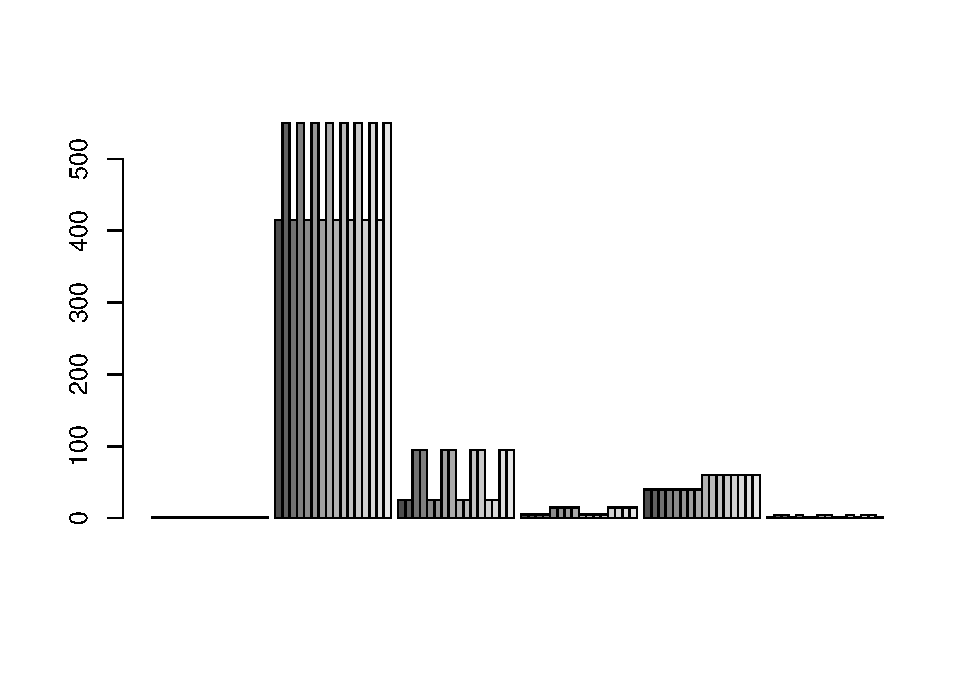
\includegraphics{Trabalho_1_SME0820_Grupo03_files/figure-latex/unnamed-chunk-4-1.pdf}
A partir do gráfico de dispersão acima parece que existe uma relação
linear entre as variáveis \(X_1\) e \(Y\). Vamos verificar tal relação a
partir do coeficiente de Pearson \(\rho\).

\textbf{Teste de Correlação de Pearson entre as variáveis \(X_1\) e
\(Y\)}

\begin{Shaded}
\begin{Highlighting}[]
\KeywordTok{cor.test}\NormalTok{(dados}\OperatorTok{$}\NormalTok{x1, dados}\OperatorTok{$}\NormalTok{y)}
\end{Highlighting}
\end{Shaded}

\begin{verbatim}
## 
##  Pearson's product-moment correlation
## 
## data:  dados$x1 and dados$y
## t = -10.086, df = 30, p-value = 3.743e-11
## alternative hypothesis: true correlation is not equal to 0
## 95 percent confidence interval:
##  -0.9395719 -0.7642987
## sample estimates:
##        cor 
## -0.8787896
\end{verbatim}

O teste de correlação de Person resultou em um \(\rho = -~0.87\) o que
indica uma forte correlação entre as variáveis. Nosso objetivo é estimar
a influência de \(X_1\) sobre \(Y\), ou seja, como \(Y\) varia em
relação às variações em \(X_1\).

\begin{Shaded}
\begin{Highlighting}[]
\NormalTok{dados }\OperatorTok
\StringTok{  }\KeywordTok{ggplot}\NormalTok{(}\KeywordTok{aes}\NormalTok{(}\DataTypeTok{x =} \StringTok{""}\NormalTok{, }\DataTypeTok{y =}\NormalTok{ dados}\OperatorTok{$}\NormalTok{x1)) }\OperatorTok{+}
\StringTok{    }\KeywordTok{geom_boxplot}\NormalTok{(}\DataTypeTok{color =} \StringTok{"blue"}\NormalTok{) }\OperatorTok{+}
\StringTok{    }\KeywordTok{stat_summary}\NormalTok{(}\DataTypeTok{fun =}\NormalTok{ mean, }\DataTypeTok{geom =} \StringTok{"point"}\NormalTok{, }\DataTypeTok{shape =} \DecValTok{20}\NormalTok{, }\DataTypeTok{size =} \DecValTok{5}\NormalTok{, }\DataTypeTok{color =} \StringTok{"red"}\NormalTok{, }\DataTypeTok{fill =} \StringTok{"red"}\NormalTok{) }\OperatorTok{+}
\StringTok{    }\KeywordTok{geom_jitter}\NormalTok{(}\DataTypeTok{color=}\StringTok{"black"}\NormalTok{, }\DataTypeTok{size=}\DecValTok{1}\NormalTok{, }\DataTypeTok{alpha=}\NormalTok{.}\DecValTok{9}\NormalTok{) }\OperatorTok{+}
\StringTok{    }\KeywordTok{theme}\NormalTok{(}\DataTypeTok{plot.title =} \KeywordTok{element_text}\NormalTok{(}\DataTypeTok{size =} \DecValTok{15}\NormalTok{, }\DataTypeTok{hjust =} \FloatTok{.5}\NormalTok{)) }\OperatorTok{+}
\StringTok{    }\KeywordTok{ggtitle}\NormalTok{(}\StringTok{"Boxplot da Variável (X1)"}\NormalTok{) }\OperatorTok{+}
\StringTok{    }\KeywordTok{xlab}\NormalTok{(}\StringTok{""}\NormalTok{) }\OperatorTok{+}\StringTok{ }\KeywordTok{ylab}\NormalTok{(}\StringTok{"Cilíndradas por Polegada Cúbica")}
\end{Highlighting}
\end{Shaded}

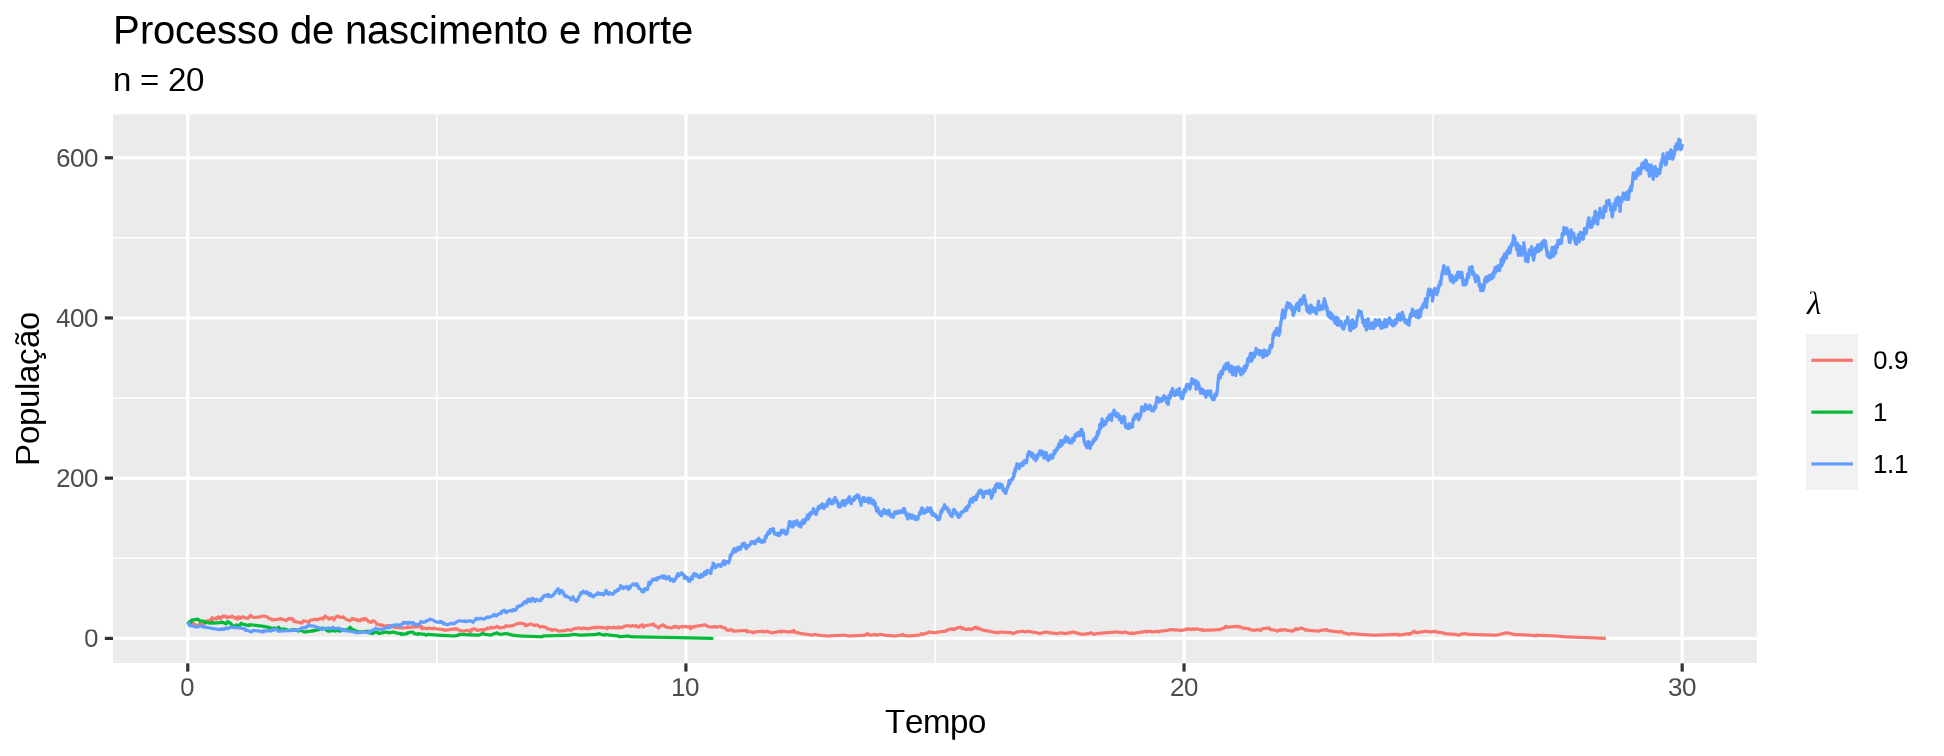
\includegraphics{Trabalho_1_SME0820_Grupo03_files/figure-latex/unnamed-chunk-6-1.pdf}
Podemos perceber a partir do boxplot acima e da função summary que
\(50\%\) dos carros tem menos de \(318\) cilíndradas.

\begin{Shaded}
\begin{Highlighting}[]
\NormalTok{dados }\OperatorTok
\StringTok{  }\KeywordTok{ggplot}\NormalTok{(}\KeywordTok{aes}\NormalTok{(}\DataTypeTok{x =} \StringTok{""}\NormalTok{, }\DataTypeTok{y =}\NormalTok{ dados}\OperatorTok{$}\NormalTok{y)) }\OperatorTok{+}
\StringTok{    }\KeywordTok{geom_boxplot}\NormalTok{(}\DataTypeTok{color =} \StringTok{"blue"}\NormalTok{) }\OperatorTok{+}
\StringTok{    }\KeywordTok{stat_summary}\NormalTok{(}\DataTypeTok{fun =}\NormalTok{ mean, }\DataTypeTok{geom =} \StringTok{"point"}\NormalTok{, }\DataTypeTok{shape =} \DecValTok{20}\NormalTok{, }\DataTypeTok{size =} \DecValTok{5}\NormalTok{, }\DataTypeTok{color =} \StringTok{"red"}\NormalTok{, }\DataTypeTok{fill =} \StringTok{"red"}\NormalTok{) }\OperatorTok{+}
\StringTok{    }\KeywordTok{geom_jitter}\NormalTok{(}\DataTypeTok{color=}\StringTok{"black"}\NormalTok{, }\DataTypeTok{size=}\DecValTok{1}\NormalTok{, }\DataTypeTok{alpha=}\NormalTok{.}\DecValTok{9}\NormalTok{) }\OperatorTok{+}
\StringTok{    }\KeywordTok{theme}\NormalTok{(}\DataTypeTok{plot.title =} \KeywordTok{element_text}\NormalTok{(}\DataTypeTok{size =} \DecValTok{15}\NormalTok{, }\DataTypeTok{hjust =} \FloatTok{.5}\NormalTok{)) }\OperatorTok{+}
\StringTok{    }\KeywordTok{ggtitle}\NormalTok{(}\StringTok{"Boxplot da Variável (Y)"}\NormalTok{) }\OperatorTok{+}
\StringTok{    }\KeywordTok{xlab}\NormalTok{(}\StringTok{""}\NormalTok{) }\OperatorTok{+}\StringTok{ }\KeywordTok{ylab}\NormalTok{(}\StringTok{"Rendimento por motor em milhas por litro"}\NormalTok{)}
\end{Highlighting}
\end{Shaded}

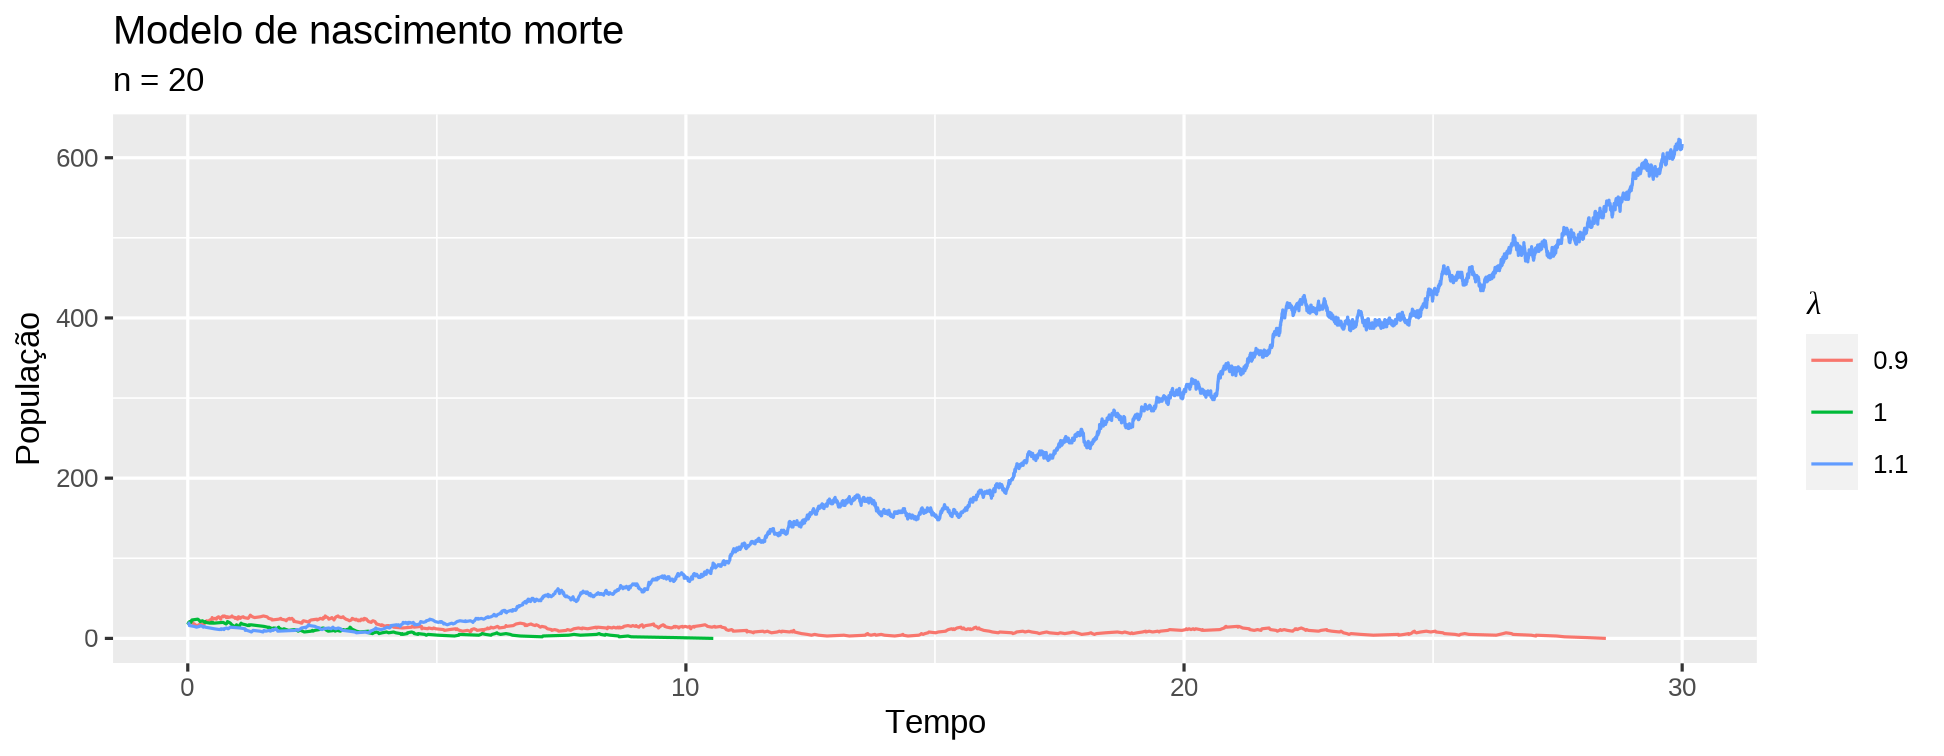
\includegraphics{Trabalho_1_SME0820_Grupo03_files/figure-latex/unnamed-chunk-7-1.pdf}
Pelo boxplot acima percebemos que os dados da variável y parecem seguir
uma distribuição Normal - o que será confirmado com a análise de um
histograma. Ainda, destaca-se quatro outliers, cujo rendimento é
superior a \(30~mi/L\).

\begin{Shaded}
\begin{Highlighting}[]
\NormalTok{dados }\OperatorTok
\StringTok{  }\KeywordTok{ggplot}\NormalTok{(}\KeywordTok{aes}\NormalTok{( }\DataTypeTok{x=}\NormalTok{dados}\OperatorTok{$}\NormalTok{y)) }\OperatorTok{+}
\StringTok{    }\KeywordTok{geom_histogram}\NormalTok{(}\KeywordTok{aes}\NormalTok{(}\DataTypeTok{y=}\NormalTok{..density..), }\DataTypeTok{color =} \StringTok{"black"}\NormalTok{, }\DataTypeTok{fill =} \StringTok{"lightblue"}\NormalTok{, }\DataTypeTok{bins =} \DecValTok{13}\NormalTok{) }\OperatorTok{+}\StringTok{ }\CommentTok{# xlab("Rendimento") + ylab("Frequência") +}
\StringTok{    }\KeywordTok{geom_vline}\NormalTok{(}\KeywordTok{aes}\NormalTok{(}\DataTypeTok{xintercept=}\KeywordTok{mean}\NormalTok{(dados}\OperatorTok{$}\NormalTok{y), }\DataTypeTok{color =} \StringTok{"Média"}\NormalTok{), }\DataTypeTok{linetype =} \StringTok{"solid"}\NormalTok{) }\OperatorTok{+}
\StringTok{    }\KeywordTok{geom_vline}\NormalTok{(}\KeywordTok{aes}\NormalTok{(}\DataTypeTok{xintercept=}\KeywordTok{median}\NormalTok{(dados}\OperatorTok{$}\NormalTok{y), }\DataTypeTok{color =} \StringTok{"Mediana"}\NormalTok{), }\DataTypeTok{linetype =} \StringTok{"solid"}\NormalTok{) }\OperatorTok{+}
\StringTok{    }\KeywordTok{labs}\NormalTok{(}\DataTypeTok{title =} \StringTok{"Histograma da variável Y ( em milhas por L)"}\NormalTok{) }\OperatorTok{+}
\StringTok{    }\KeywordTok{scale_x_continuous}\NormalTok{(}\StringTok{"Rendimento"}\NormalTok{, }\DataTypeTok{breaks =} \KeywordTok{seq}\NormalTok{(}\DecValTok{10}\NormalTok{,}\DecValTok{38}\NormalTok{,}\DecValTok{2}\NormalTok{)) }\OperatorTok{+}
\StringTok{    }\KeywordTok{scale_y_continuous}\NormalTok{(}\StringTok{"Frequência Relativa"}\NormalTok{) }\OperatorTok{+}
\StringTok{    }\KeywordTok{scale_color_manual}\NormalTok{(}\DataTypeTok{name=}\StringTok{" "}\NormalTok{, }\DataTypeTok{values =} \KeywordTok{c}\NormalTok{(}\StringTok{"red"}\NormalTok{, }\StringTok{"black"}\NormalTok{)) }\OperatorTok{+}
\StringTok{    }\KeywordTok{ylab}\NormalTok{(}\StringTok{"Frequência") +}
\StringTok{    theme(plot.title = element_text(hjust = 0.5)) +}
\StringTok{    theme_pubclean()}
\end{Highlighting}
\end{Shaded}

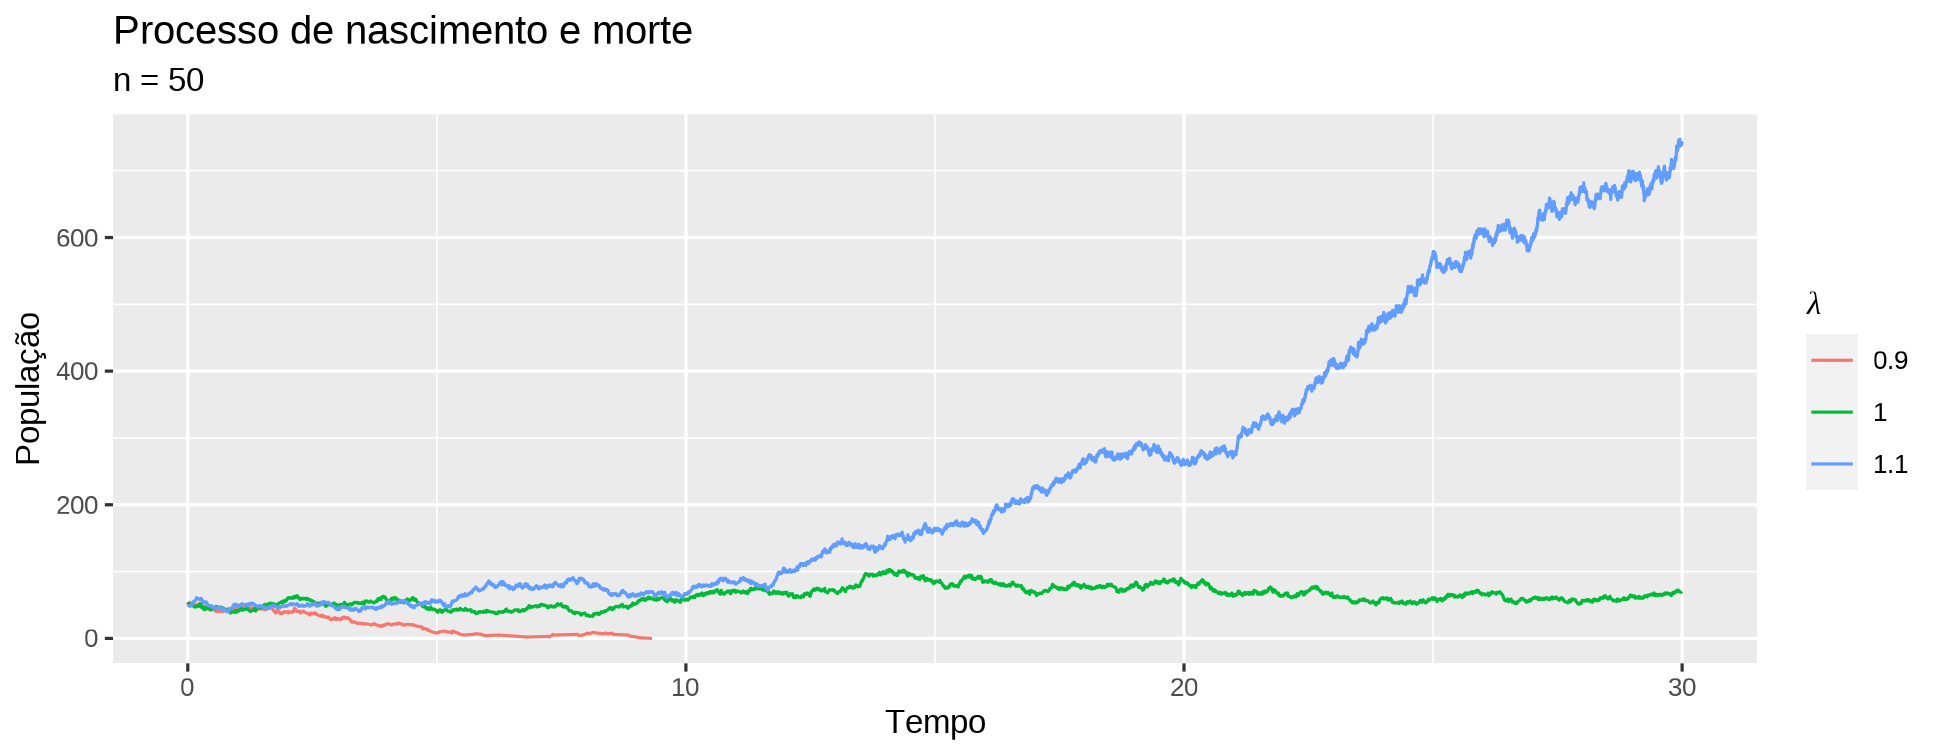
\includegraphics{Trabalho_1_SME0820_Grupo03_files/figure-latex/unnamed-chunk-8-1.pdf}
O histograma acima representa a distribuição da variável y. Fica claro,
portanto, que os dados da variável resposta se assemelham a uma
distribuição normal, não fossem os outliers.

\begin{Shaded}
\begin{Highlighting}[]
\NormalTok{dados }\OperatorTok
\StringTok{  }\KeywordTok{select}\NormalTok{(y,x1) }\OperatorTok
\StringTok{  }\KeywordTok{filter}\NormalTok{(y}\OperatorTok{>}\DecValTok{30}\NormalTok{) }\OperatorTok
\StringTok{  }\KeywordTok{kable}\NormalTok{(}\DataTypeTok{caption =} \StringTok{"Tabela com os 4 outliers presentes nos valores de Y"}\NormalTok{)}
\end{Highlighting}
\end{Shaded}

\begin{longtable}[]{@{}rr@{}}
\caption{Tabela com os 4 outliers presentes nos valores de
Y}\tabularnewline
\toprule
y & x1\tabularnewline
\midrule
\endfirsthead
\toprule
y & x1\tabularnewline
\midrule
\endhead
34.7 & 89.7\tabularnewline
30.4 & 96.9\tabularnewline
36.5 & 85.3\tabularnewline
31.9 & 96.9\tabularnewline
\bottomrule
\end{longtable}

A partir do histograma e da tabela acima, concluimos que os 4 outliers
referem-se aos valores: \(30.4\), \(31.9\), \(34.7\), e \(36.5\).

Vamos verificar a distribuição da variável \(X_1\)

\begin{Shaded}
\begin{Highlighting}[]
\NormalTok{dados }\OperatorTok
\StringTok{  }\KeywordTok{ggplot}\NormalTok{(}\KeywordTok{aes}\NormalTok{( }\DataTypeTok{x=}\NormalTok{dados}\OperatorTok{$}\NormalTok{x1)) }\OperatorTok{+}
\StringTok{    }\KeywordTok{geom_histogram}\NormalTok{(}\KeywordTok{aes}\NormalTok{(}\DataTypeTok{y=}\NormalTok{..density..), }\DataTypeTok{color =} \StringTok{"black"}\NormalTok{, }\DataTypeTok{fill =} \StringTok{"lightgreen"}\NormalTok{, }\DataTypeTok{bins =} \DecValTok{15}\NormalTok{) }\OperatorTok{+}\StringTok{ }\CommentTok{# xlab("Rendimento") + ylab("Frequência") +}
\StringTok{    }\KeywordTok{geom_vline}\NormalTok{(}\KeywordTok{aes}\NormalTok{(}\DataTypeTok{xintercept=}\KeywordTok{mean}\NormalTok{(dados}\OperatorTok{$}\NormalTok{x1), }\DataTypeTok{color =} \StringTok{"Média"}\NormalTok{), }\DataTypeTok{linetype =} \StringTok{"solid"}\NormalTok{) }\OperatorTok{+}
\StringTok{    }\KeywordTok{geom_vline}\NormalTok{(}\KeywordTok{aes}\NormalTok{(}\DataTypeTok{xintercept=}\KeywordTok{median}\NormalTok{(dados}\OperatorTok{$}\NormalTok{x1), }\DataTypeTok{color =} \StringTok{"Mediana"}\NormalTok{), }\DataTypeTok{linetype =} \StringTok{"solid"}\NormalTok{) }\OperatorTok{+}
\StringTok{    }\KeywordTok{labs}\NormalTok{(}\DataTypeTok{title =} \StringTok{"Histograma da variável X1 (Cilindradas por Polegada Cúbica)"}\NormalTok{) }\OperatorTok{+}
\StringTok{    }\KeywordTok{scale_x_continuous}\NormalTok{(}\StringTok{"Cilindradas"}\NormalTok{, }\DataTypeTok{breaks =} \KeywordTok{c}\NormalTok{(}\DecValTok{100}\NormalTok{,}\DecValTok{150}\NormalTok{,}\DecValTok{200}\NormalTok{,}\DecValTok{250}\NormalTok{,}\DecValTok{300}\NormalTok{,}\DecValTok{350}\NormalTok{,}\DecValTok{400}\NormalTok{,}\DecValTok{450}\NormalTok{,}\DecValTok{500}\NormalTok{)) }\OperatorTok{+}
\StringTok{    }\KeywordTok{scale_y_continuous}\NormalTok{(}\StringTok{"Frequência relativa"}\NormalTok{) }\OperatorTok{+}
\StringTok{  }\KeywordTok{scale_color_manual}\NormalTok{(}\DataTypeTok{name=}\StringTok{" "}\NormalTok{, }\DataTypeTok{values =} \KeywordTok{c}\NormalTok{(}\StringTok{"red"}\NormalTok{, }\StringTok{"black"}\NormalTok{))}\OperatorTok{+}
\StringTok{  }\CommentTok{#limits = c(85,500,1)) +}
\StringTok{    }\KeywordTok{ylab}\NormalTok{(}\StringTok{"Frequência") +}
\StringTok{    theme(plot.title = element_text(hjust = 0.5)) +}
\StringTok{    theme_pubclean()}
\end{Highlighting}
\end{Shaded}

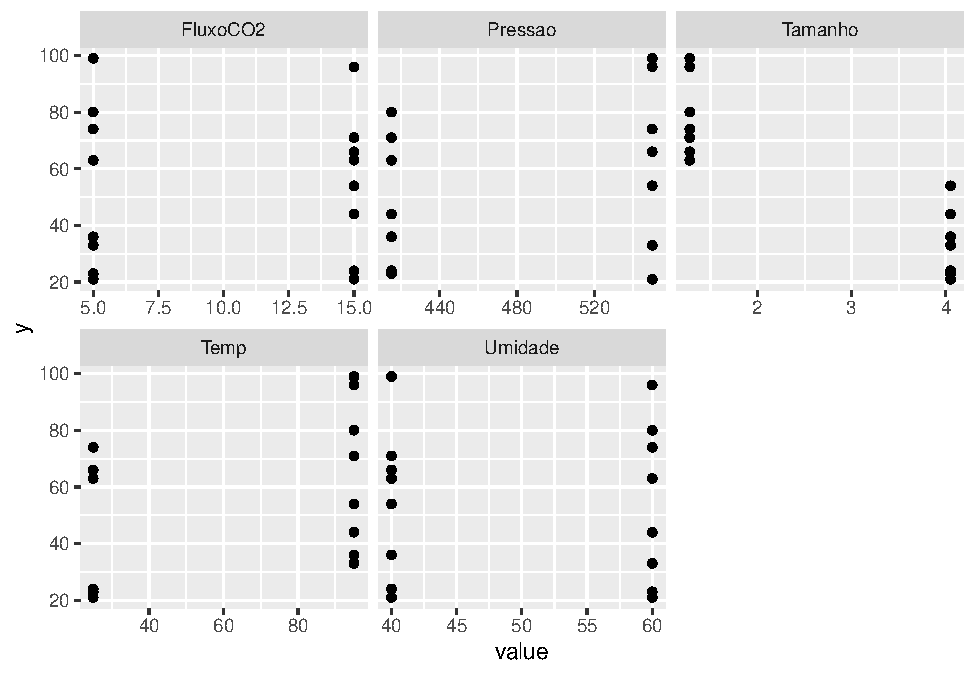
\includegraphics{Trabalho_1_SME0820_Grupo03_files/figure-latex/unnamed-chunk-10-1.pdf}
O histograma da variável \(X_1\) não apresenta uma distribuição bem
definida, entretanto, destaca-se maior frequência para os valores em
torno de \(350\) cilíndradas.

\textbf{Moda dos valores de \(X_1\)}

\begin{Shaded}
\begin{Highlighting}[]
\NormalTok{getmode <-}\StringTok{ }\ControlFlowTok{function}\NormalTok{(v) \{}
\NormalTok{   uniqv <-}\StringTok{ }\KeywordTok{unique}\NormalTok{(v)}
\NormalTok{   uniqv[}\KeywordTok{which.max}\NormalTok{(}\KeywordTok{tabulate}\NormalTok{(}\KeywordTok{match}\NormalTok{(v, uniqv)))]}
\NormalTok{\}}
   
\NormalTok{mode_x1 =}\StringTok{ }\KeywordTok{getmode}\NormalTok{(dados}\OperatorTok{$}\NormalTok{x1)}
\KeywordTok{print}\NormalTok{(mode_x1)}
\end{Highlighting}
\end{Shaded}

\begin{verbatim}
## [1] 350
\end{verbatim}

De fato, a moda para os valores de \(X_1\) é \(350\).

\hypertarget{parte-b}{%
\subsection{\texorpdfstring{Parte
\textbf{b)}:}{Parte b):}}\label{parte-b}}

Consultar e descrever brevemente os conceitos Data splitting, cross
validation, overfitting, underfitting, missing data, encoding data.

\begin{enumerate}
\def\labelenumi{\arabic{enumi}.}
\item
  \textbf{Data Splitting}: Data Splitting ou também ``divisão de dados''
  é uma abordagem para proteger dados confidenciais de acesso não
  autorizado, criptografando os dados e armazenando diferentes partes de
  um arquivo em servidores diferentes. Quando os dados divididos são
  acessados, as partes são recuperadas, combinadas e descriptografadas.
\item
  \textbf{Cross Validation}: Cross Validation ou também ``validação
  cruzada'' é uma técnica muito utilizada para avaliar o desempenho de
  modelos de aprendizado de máquina. Consiste, basicamente, em
  particionar os dados em conjuntos, onde um conjunto é utilizado para
  treino e outro para teste e avaliação do desempenho do modelo. A
  utilização correta da técnica tem altas chances de detectar se um
  modelo está sobreajustado aos seus dados de treinamento, ou seja,
  sofrendo overfitting. Vale ressaltar que existem vários métodos de
  aplicação da validação cruzada.
\item
  \textbf{Overfitting}: Overfitting ou também ``Sobreajuste'' consiste
  na situação em que o modelo se ajusta bem demais ao conjunto de
  treinamento. Ou seja, nos dados de treinamento, em geral, a acurácia
  do modelo é muito alta (e, quando há 100\% de acurácia dizemos que o
  modelo ``memorizou'' os dados). Isso ocorre pois além de aprender os
  detalhes dos dados o modelo também aprende os ruídos, o que prejudica
  sua capacidade de generalização no conjunto de teste. Em geral, quanto
  maior a complexidade do modelo mais propenso ao Overfitting ele se
  torna.
\item
  \textbf{Underfitting}: Já o Underfitting, por outro lado, refere-se ao
  problema em que o modelo não é capaz de modelar o conjunto de
  treinamento e nem generalizar para dados nunca vistos. Em geral, a
  solução reside no aumento da complexidade do modelo ou a troca do
  algoritmo.
\item
  \textbf{Missing data}: Missing data, muitas vezes referido como
  missing values (com tradução literal: valores que faltam), é um
  conceito utilizado para quando alguma(s) observação(ões) no conjunto
  de dados está(ão) vazia(s), causando ambuiguidade e falta de precisão
  para a análise do mesmo. Na análise multivariada, temos uma relação
  proporcional da quantidade de variáveis a serem relacionadas com a
  falta de rigor causada pelos missing values.
\item
  \textbf{Encoding data}: Encoding data (de tradução literal: dados
  codificados) é o nome dado para o processo de converter dados para um
  formato específico, assegurando sua transmissão e otimizando o modelo.
  Seu processo inverso - ou seja, a decodificação - refere-se a extrair
  as informações da forma convertida.
\end{enumerate}

\hypertarget{parte-c}{%
\subsection{\texorpdfstring{Parte
\textbf{c)}:}{Parte c):}}\label{parte-c}}

\begin{enumerate}
\def\labelenumi{\arabic{enumi}.}
\tightlist
\item
  Calcular \(S_{XX}\),\(S_{YY}\) e \(S_{XY}\)
\end{enumerate}

Calculando o valor de \(S_{xx}\)

\[S_{XX} =  \sum_{i=1}^n (x -\bar{x})^2\]

\begin{Shaded}
\begin{Highlighting}[]
\NormalTok{xbarra=}\KeywordTok{mean}\NormalTok{(x1)}
\NormalTok{x1}\OperatorTok{-}\NormalTok{xbarra}
\end{Highlighting}
\end{Shaded}

\begin{verbatim}
##  [1]   67.62857  -32.37143   68.62857  157.62857  -51.37143  -20.37143
##  [7] -192.67143 -185.47143   67.62857 -197.07143 -111.37143  -24.37143
## [13] -142.37143   19.62857  157.62857   67.62857   35.62857  -51.37143
## [19]   77.62857  117.62857 -185.47143  177.62857 -148.77143   35.62857
## [25]   68.62857   68.62857   77.62857   77.62857
\end{verbatim}

\begin{Shaded}
\begin{Highlighting}[]
\NormalTok{(x1}\OperatorTok{-}\NormalTok{xbarra)}\OperatorTok{^}\DecValTok{2}
\end{Highlighting}
\end{Shaded}

\begin{verbatim}
##  [1]  4573.6237  1047.9094  4709.8808 24846.7665  2639.0237   414.9951
##  [7] 37122.2794 34399.6508  4573.6237 38837.1480 12403.5951   593.9665
## [13] 20269.6237   385.2808 24846.7665  4573.6237  1269.3951  2639.0237
## [19]  6026.1951 13836.4808 34399.6508 31551.9094 22132.9380  1269.3951
## [25]  4709.8808  4709.8808  6026.1951  6026.1951
\end{verbatim}

\begin{Shaded}
\begin{Highlighting}[]
\NormalTok{Sxx=}\KeywordTok{sum}\NormalTok{((x1}\OperatorTok{-}\NormalTok{xbarra)}\OperatorTok{^}\DecValTok{2}\NormalTok{)}
\end{Highlighting}
\end{Shaded}

\hypertarget{calculando-o-valor-de-s_yy}{%
\subsubsection{\texorpdfstring{Calculando o valor de
\(S_{yy}\)}{Calculando o valor de S\_\{yy\}}}\label{calculando-o-valor-de-s_yy}}

\[S_{YY} =  \sum_{i=1}^n (y - \bar{y})^2\]

\begin{Shaded}
\begin{Highlighting}[]
\NormalTok{ybarra=}\KeywordTok{mean}\NormalTok{(y)}
\NormalTok{y}\OperatorTok{-}\NormalTok{ybarra}
\end{Highlighting}
\end{Shaded}

\begin{verbatim}
##  [1] -3.1564286 -0.1564286 -1.9064286 -8.9564286  1.9635714  1.3135714
##  [7] 14.5435714 10.2435714 -3.6564286 16.3435714  1.3435714 -0.4564286
## [13]  0.1435714 -2.3564286 -5.2664286 -2.3564286 -3.7464286  3.3835714
## [19]  1.3135714 -3.5664286 11.7435714 -6.8864286  3.7435714 -0.4264286
## [25] -6.2564286 -6.8864286 -6.3864286 -3.6564286
\end{verbatim}

\begin{Shaded}
\begin{Highlighting}[]
\NormalTok{(y}\OperatorTok{-}\NormalTok{ybarra)}\OperatorTok{^}\DecValTok{2}
\end{Highlighting}
\end{Shaded}

\begin{verbatim}
##  [1]   9.96304133   0.02446990   3.63446990  80.21761276   3.85561276
##  [6]   1.72546990 211.51546990 104.93075561  13.36946990 267.11232704
## [11]   1.80518418   0.20832704   0.02061276   5.55275561  27.73526990
## [16]   5.55275561  14.03572704  11.44855561   1.72546990  12.71941276
## [21] 137.91146990  47.42289847  14.01432704   0.18184133  39.14289847
## [26]  47.42289847  40.78646990  13.36946990
\end{verbatim}

\begin{Shaded}
\begin{Highlighting}[]
\NormalTok{Syy=}\KeywordTok{sum}\NormalTok{((y}\OperatorTok{-}\NormalTok{ybarra)}\OperatorTok{^}\DecValTok{2}\NormalTok{)}
\end{Highlighting}
\end{Shaded}

\hypertarget{calculando-o-valor-de-s_xy}{%
\subsubsection{\texorpdfstring{Calculando o valor de
\(S_{xy}\)}{Calculando o valor de S\_\{xy\}}}\label{calculando-o-valor-de-s_xy}}

\[S_{XY} =  \sum_{i=1}^n (x - \bar{x})(y - \bar{y})\]

\begin{Shaded}
\begin{Highlighting}[]
\NormalTok{Sxy=}\KeywordTok{sum}\NormalTok{((x1}\OperatorTok{-}\NormalTok{xbarra)}\OperatorTok{*}\NormalTok{(y}\OperatorTok{-}\NormalTok{ybarra))}
\KeywordTok{cbind}\NormalTok{(Sxx,Syy,Sxy)}
\end{Highlighting}
\end{Shaded}

\begin{verbatim}
##           Sxx      Syy      Sxy
## [1,] 350834.9 1117.405 -17523.4
\end{verbatim}

\begin{enumerate}
\def\labelenumi{\arabic{enumi}.}
\setcounter{enumi}{1}
\tightlist
\item
  Ajustar um modelo de regressão linear simples, apresentar a estimativa
  de \(\beta_0, \beta_1\) e \(\sigma^2\) e fazer um gráfico com a reta
  ajustada
\end{enumerate}

\hypertarget{estimacao-dos-parametros}{%
\subsection{Estimacao dos parametros}\label{estimacao-dos-parametros}}

\[\beta_1 = S_{XY}/S_{XX}\]

\hypertarget{calculando-o-valor-do-coeficiente-angular-beta_1}{%
\subsubsection{\texorpdfstring{Calculando o valor do coeficiente angular
\(\beta_1\)}{Calculando o valor do coeficiente angular \textbackslash beta\_1}}\label{calculando-o-valor-do-coeficiente-angular-beta_1}}

\begin{Shaded}
\begin{Highlighting}[]
\NormalTok{b1_est <-}\StringTok{ }\NormalTok{Sxy}\OperatorTok{/}\NormalTok{Sxx}
\end{Highlighting}
\end{Shaded}

\hypertarget{calculando-o-valor-do-intercepto-beta_0}{%
\subsubsection{\texorpdfstring{Calculando o valor do intercepto
\(\beta_0\)}{Calculando o valor do intercepto \textbackslash beta\_0}}\label{calculando-o-valor-do-intercepto-beta_0}}

\begin{Shaded}
\begin{Highlighting}[]
\NormalTok{b0_est <-}\StringTok{ }\KeywordTok{mean}\NormalTok{(y) }\OperatorTok{-}\StringTok{ }\NormalTok{b1_est}\OperatorTok{*}\KeywordTok{mean}\NormalTok{(x1)}
\end{Highlighting}
\end{Shaded}

\hypertarget{calculando-o-estimador-de-sigma2-nuxe3o-viesado.}{%
\subsubsection{\texorpdfstring{Calculando o estimador de \(\sigma^2\)
não
viesado.}{Calculando o estimador de \textbackslash sigma\^{}2 não viesado.}}\label{calculando-o-estimador-de-sigma2-nuxe3o-viesado.}}

Tal estimador é obtido através da soma do quadrado dos resíduos,
definido pela variável \emph{QMres}, de modo que:

\begin{Shaded}
\begin{Highlighting}[]
\CommentTok{# Soma do quadrado da regressão:}
\NormalTok{SQreg <-}\StringTok{ }\NormalTok{b1_est}\OperatorTok{*}\NormalTok{Sxy}
\CommentTok{# Soma do quadrado total:}
\NormalTok{SQtotal <-}\StringTok{ }\KeywordTok{sum}\NormalTok{((y}\OperatorTok{-}\KeywordTok{mean}\NormalTok{(y))}\OperatorTok{^}\DecValTok{2}\NormalTok{)}
\CommentTok{# Diferença entre a soma do quadrado da regressão e a soma do quadrado total:}
\NormalTok{SQres <-}\StringTok{ }\NormalTok{SQtotal }\OperatorTok{-}\StringTok{ }\NormalTok{SQreg}
\CommentTok{# Soma do quadrado dos resíduos:}
\NormalTok{QMres <-}\StringTok{ }\NormalTok{SQres}\OperatorTok{/}\NormalTok{(n}\DecValTok{-2}\NormalTok{)}
\end{Highlighting}
\end{Shaded}

\begin{Shaded}
\begin{Highlighting}[]
\NormalTok{dados }\OperatorTok\StringTok{ }\KeywordTok{ggplot}\NormalTok{(}\KeywordTok{aes}\NormalTok{(}\DataTypeTok{x=}\NormalTok{ x1, }\DataTypeTok{y=}\NormalTok{ y)) }\OperatorTok{+}\StringTok{ }\KeywordTok{geom_point}\NormalTok{() }\OperatorTok{+}
\StringTok{  }\KeywordTok{geom_smooth}\NormalTok{(}\DataTypeTok{method=}\StringTok{'lm'}\NormalTok{, }\DataTypeTok{formula=}\NormalTok{ y}\OperatorTok{~}\NormalTok{x) }\OperatorTok{+}
\StringTok{  }\KeywordTok{theme_pubclean}\NormalTok{()}
\end{Highlighting}
\end{Shaded}

\includegraphics{Trabalho_1_SME0820_Grupo03_files/figure-latex/unnamed-chunk-18-1.pdf}

\begin{Shaded}
\begin{Highlighting}[]
\CommentTok{#Arredondando b0 e b1}
\KeywordTok{round}\NormalTok{(b0_est, }\DecValTok{4}\NormalTok{)}
\end{Highlighting}
\end{Shaded}

\begin{verbatim}
## [1] 34.2602
\end{verbatim}

\begin{Shaded}
\begin{Highlighting}[]
\KeywordTok{round}\NormalTok{(b1_est, }\DecValTok{4}\NormalTok{)}
\end{Highlighting}
\end{Shaded}

\begin{verbatim}
## [1] -0.0499
\end{verbatim}

Consequentemente, a reta ajustada é:
\[\widehat{Y}_i=1224.043-0.7769X_i\]

\begin{enumerate}
\def\labelenumi{\arabic{enumi}.}
\setcounter{enumi}{2}
\tightlist
\item
  Calcule o valor dos \(\hat{Y}\) e o valor dos resíduos para seu
  modelo, resumo e histograma dos resíduos, e faça uma análise da
  distribuição destes.
\end{enumerate}

O cálculo de \(\hat{Y}\) pode ser realizado utilizando o modelo de
regressão linear simples, em que a variabilidade de interesse é dada em
função de uma única covariável - no caso, \emph{x1}. No R, podemos
expressar \(\hat{Y}\) como sendo:

\begin{Shaded}
\begin{Highlighting}[]
\NormalTok{y_pred <-}\StringTok{  }\NormalTok{b0_est }\OperatorTok{+}\StringTok{ }\NormalTok{b1_est}\OperatorTok{*}\NormalTok{x1}
\end{Highlighting}
\end{Shaded}

Os resíduos se dão pelo desvio entre as observações e os valores
preditos, sendo uma medida de variabilidade na variável resposta onde
qualquer desvio relativo a suposição dos erros deveria aparecer.
Analisá-los nos permite um discernimento maior em relação a quão
adequado é o modelo. Fazendo uso do cálculo de \emph{y\_pred} feito
anteriormente, salvamos nossos resíduos em uma variável \emph{res}
abaixo.

\begin{Shaded}
\begin{Highlighting}[]
\NormalTok{res <-}\StringTok{ }\NormalTok{y }\OperatorTok{-}\StringTok{ }\NormalTok{y_pred}
\end{Highlighting}
\end{Shaded}

Utilizando o comando \emph{summary}, podemos observar as principais
medidas descritivas da variável, o que nos auxilia para a análise da
mesma.

\begin{Shaded}
\begin{Highlighting}[]
\KeywordTok{tibble}\NormalTok{(}\KeywordTok{summary}\NormalTok{(res)) }\OperatorTok\StringTok{ }\KeywordTok{kable}\NormalTok{(}\DataTypeTok{caption =} \StringTok{"Principais medidas descritivas dos resíduos"}\NormalTok{)}
\end{Highlighting}
\end{Shaded}

\begin{longtable}[]{@{}r@{}}
\caption{Principais medidas descritivas dos resíduos}\tabularnewline
\toprule
summary(res)\tabularnewline
\midrule
\endfirsthead
\toprule
summary(res)\tabularnewline
\midrule
\endhead
-6.9676\tabularnewline
-1.8217\tabularnewline
0.2212\tabularnewline
0.0000\tabularnewline
1.6375\tabularnewline
6.5003\tabularnewline
\bottomrule
\end{longtable}

Também podemos construir um histograma, assim como um gráfico
quantil-quantil, que facilitará a visualização do comportamento dos
resíduos.

\begin{Shaded}
\begin{Highlighting}[]
\CommentTok{# Histograma}
\NormalTok{n_res <-}\StringTok{ }\KeywordTok{length}\NormalTok{(res)}
\NormalTok{normalDist<-}\StringTok{ }\KeywordTok{rnorm}\NormalTok{(}\KeywordTok{length}\NormalTok{(res), }\DataTypeTok{mean =}  \KeywordTok{mean}\NormalTok{(res), }\DataTypeTok{sd=} \KeywordTok{sd}\NormalTok{(res))}
\NormalTok{dat<-}\StringTok{ }\KeywordTok{data.frame}\NormalTok{(}\DataTypeTok{error =}\NormalTok{ res, }\DataTypeTok{norm =}\NormalTok{ normalDist)}
\KeywordTok{ggplot}\NormalTok{(}\KeywordTok{tibble}\NormalTok{(res), }\KeywordTok{aes}\NormalTok{(}\DataTypeTok{x =}\NormalTok{ res)) }\OperatorTok{+}
\StringTok{  }\KeywordTok{ylab}\NormalTok{(}\StringTok{"Frequência") +}
\StringTok{  geom_histogram(aes(y=..density..), color = "}\NormalTok{black}\StringTok{", fill = "}\CommentTok{#FF69B4", bins=12, position="identity")+}
  \KeywordTok{labs}\NormalTok{(}\DataTypeTok{title =} \StringTok{"Histograma dos resíduos"}\NormalTok{)}\OperatorTok{+}
\StringTok{  }\KeywordTok{geom_density}\NormalTok{(}\DataTypeTok{data =}\NormalTok{ dat) }\OperatorTok{+}
\StringTok{  }\KeywordTok{scale_x_continuous}\NormalTok{(}\StringTok{"Resíduos"}\NormalTok{, }\DataTypeTok{limits =} \KeywordTok{c}\NormalTok{(}\OperatorTok{-}\DecValTok{8}\NormalTok{,}\DecValTok{8}\NormalTok{,}\DecValTok{1}\NormalTok{), }\DataTypeTok{breaks =} \KeywordTok{c}\NormalTok{(}\OperatorTok{-}\DecValTok{8}\OperatorTok{:}\DecValTok{8}\NormalTok{))}\OperatorTok{+}
\StringTok{  }\KeywordTok{theme}\NormalTok{(}\DataTypeTok{plot.title =} \KeywordTok{element_text}\NormalTok{(}\DataTypeTok{hjust =} \FloatTok{0.5}\NormalTok{)) }\OperatorTok{+}
\StringTok{  }\KeywordTok{theme_classic}\NormalTok{()}
\end{Highlighting}
\end{Shaded}

\includegraphics{Trabalho_1_SME0820_Grupo03_files/figure-latex/unnamed-chunk-23-1.pdf}

\begin{Shaded}
\begin{Highlighting}[]
\CommentTok{# Q-Q}
\KeywordTok{qqnorm}\NormalTok{(res, }\DataTypeTok{main =} \StringTok{"Q-Q Plot da Normal com os resíduos"}\NormalTok{, }\DataTypeTok{ylab =}\StringTok{" Quantis dos resíduos "}\NormalTok{, }\DataTypeTok{xlab =} \StringTok{" Quantis da Normal "}\NormalTok{)}
\KeywordTok{qqline}\NormalTok{(res, }\DataTypeTok{col =} \StringTok{"#FF69B4"}\NormalTok{)}
\end{Highlighting}
\end{Shaded}

\includegraphics{Trabalho_1_SME0820_Grupo03_files/figure-latex/qqplotresidu-1.pdf}

Desse modo, é possível observar que os resíduos tendem a se aproximar
cada vez mais da normal. Posteriormente, a normalidade dos resíduos será
abordada com mais precisão.

\begin{enumerate}
\def\labelenumi{\arabic{enumi}.}
\setcounter{enumi}{3}
\tightlist
\item
  testes de hipotese para \(\beta_0\) e \(\beta_1\)
\end{enumerate}

Para realizarmos nossos testes de hipóteses, é necessário o estimador do
parâmetro \(\sigma^2\) do nosso modelo, uma vez que ele não é dado. Tal
estimador não viesado é obtido através da soma do quadrado dos resíduos,
definido pela variável \emph{QMres}, calculada no item 3 de modo que:

\begin{Shaded}
\begin{Highlighting}[]
\CommentTok{# Soma do quadrado da regressão:}
\NormalTok{SQreg <-}\StringTok{ }\NormalTok{b1_est}\OperatorTok{*}\NormalTok{Sxy}
\CommentTok{# Soma do quadrado total:}
\NormalTok{SQtotal <-}\StringTok{ }\KeywordTok{sum}\NormalTok{((y}\OperatorTok{-}\KeywordTok{mean}\NormalTok{(y))}\OperatorTok{^}\DecValTok{2}\NormalTok{)}
\CommentTok{# Diferença entre a soma do quadrado da regressão e a soma do quadrado total:}
\NormalTok{SQres <-}\StringTok{ }\NormalTok{SQtotal }\OperatorTok{-}\StringTok{ }\NormalTok{SQreg}
\CommentTok{# Soma do quadrado dos resíduos:}
\NormalTok{QMres <-}\StringTok{ }\NormalTok{SQres}\OperatorTok{/}\NormalTok{(n}\DecValTok{-2}\NormalTok{)}
\end{Highlighting}
\end{Shaded}

A partir disso, podemos prosseguir com nossos testes de hipóteses para
\(\beta_1\) e \(\beta_0\), com decisão de rejeitar ou não \(H_0\), uma
vez que este representa o parâmetro se igualar a 0 estatisticamente caso
não seja rejeitado, descrevendo a significância da contribuição do
mesmo.

\begin{itemize}
\tightlist
\item
  Testagem se \(\beta_1 = 0\):
\end{itemize}

\(\beta_1\) possuí distribuição Normal com média \(\beta_1\) e variância
\(\sigma^2/S_{xx}\), com isso, definimos:

\begin{Shaded}
\begin{Highlighting}[]
\NormalTok{dp_b1 <-}\StringTok{ }\NormalTok{(}\KeywordTok{sqrt}\NormalTok{(QMres}\OperatorTok{/}\NormalTok{Sxx))}
\NormalTok{t0_b1 <-}\StringTok{ }\NormalTok{b1_est}\OperatorTok{/}\NormalTok{dp_b1}
\end{Highlighting}
\end{Shaded}

Pelo enunciado, é dado que \(\alpha= 5\%\). Se H0 não for rejeitado,
temos que \(\beta_1\) é estatisticamente igual a zero. A partir disso,
definimos \(\alpha\) e dois quantis, de modo que \emph{t1} é o quantil
\(\frac{\alpha}{2}\) da distribuicao \(t\) com grau de liberdade \$ n
-2\$, enquanto \emph{t2} é o quantil \(\frac{1-\alpha}{2}\) da
distribuicao \(t\) com grau de liberdade \(n -2\). Com esses dados,
podemos construir nosso programa de decisão que retornará caso \(H_0\)
seja rejeitado.

\begin{Shaded}
\begin{Highlighting}[]
\NormalTok{alpha <-}\StringTok{ }\FloatTok{0.05}
\NormalTok{t1 <-}\StringTok{ }\KeywordTok{qt}\NormalTok{(alpha}\OperatorTok{/}\DecValTok{2}\NormalTok{,n}\DecValTok{-2}\NormalTok{)}
\NormalTok{t2 <-}\StringTok{ }\KeywordTok{qt}\NormalTok{(}\DecValTok{1}\OperatorTok{-}\NormalTok{alpha}\OperatorTok{/}\DecValTok{2}\NormalTok{,n}\DecValTok{-2}\NormalTok{)}
\ControlFlowTok{if}\NormalTok{(t0_b1 }\OperatorTok{<}\StringTok{ }\NormalTok{t1 }\OperatorTok{||}\StringTok{ }\NormalTok{t0_b1}\OperatorTok{>}\NormalTok{t2)\{}
  \KeywordTok{cat}\NormalTok{(}\StringTok{"Rejeita-se H0"}\NormalTok{)}
\NormalTok{\}}
\end{Highlighting}
\end{Shaded}

\begin{verbatim}
## Rejeita-se H0
\end{verbatim}

Para \(\alpha= 1\%\):

\begin{Shaded}
\begin{Highlighting}[]
\NormalTok{alpha <-}\StringTok{ }\FloatTok{0.01}
\NormalTok{t1 <-}\StringTok{ }\KeywordTok{qt}\NormalTok{(alpha}\OperatorTok{/}\DecValTok{2}\NormalTok{,n}\DecValTok{-2}\NormalTok{)}
\NormalTok{t2 <-}\StringTok{ }\KeywordTok{qt}\NormalTok{(}\DecValTok{1}\OperatorTok{-}\NormalTok{alpha}\OperatorTok{/}\DecValTok{2}\NormalTok{,n}\DecValTok{-2}\NormalTok{)}
\ControlFlowTok{if}\NormalTok{(t0_b1 }\OperatorTok{<}\StringTok{ }\NormalTok{t1 }\OperatorTok{||}\StringTok{ }\NormalTok{t0_b1}\OperatorTok{>}\NormalTok{t2)\{}
  \KeywordTok{cat}\NormalTok{(}\StringTok{"Rejeita-se H0"}\NormalTok{)}
\NormalTok{\}}
\end{Highlighting}
\end{Shaded}

\begin{verbatim}
## Rejeita-se H0
\end{verbatim}

Realizando o teste, temos que H0 é rejeitado, logo, \(\beta_1\) é
diferente de zero.

\begin{itemize}
\tightlist
\item
  Testagem se \(\beta_0 = 0\):
\end{itemize}

\(\beta_0\) possuí distribuição Normal com média \(\beta_0\) e variância
\(\sigma^2((\frac{1}{n})+\frac{\bar{X}}{S_{xx}}))\), com isso,
definimos:

\begin{Shaded}
\begin{Highlighting}[]
\NormalTok{dp_b0 <-}\StringTok{ }\NormalTok{(}\KeywordTok{sqrt}\NormalTok{( QMres }\OperatorTok{*}\NormalTok{( (}\DecValTok{1}\OperatorTok{/}\NormalTok{n) }\OperatorTok{+}\StringTok{ }\NormalTok{(}\KeywordTok{mean}\NormalTok{(x1))}\OperatorTok{^}\DecValTok{2}\OperatorTok{/}\NormalTok{Sxx )))}
\NormalTok{t0_b0 <-}\StringTok{ }\NormalTok{b0_est}\OperatorTok{/}\NormalTok{dp_b0}
\end{Highlighting}
\end{Shaded}

Em um processo semelhante à testagem de \(\beta_1\), com \(\alpha\)= 5\%
e os mesmos quantis, também é possível a construção de nossa função de
decisão. Se H0 não for rejeitado, temos que \(\beta_0\) é
estatisticamente igual a zero.

\begin{Shaded}
\begin{Highlighting}[]
\NormalTok{alpha <-}\StringTok{ }\FloatTok{0.05}
\NormalTok{t1 <-}\StringTok{ }\KeywordTok{qt}\NormalTok{(alpha}\OperatorTok{/}\DecValTok{2}\NormalTok{,n}\DecValTok{-2}\NormalTok{)}
\NormalTok{t2 <-}\StringTok{ }\KeywordTok{qt}\NormalTok{(}\DecValTok{1}\OperatorTok{-}\NormalTok{alpha}\OperatorTok{/}\DecValTok{2}\NormalTok{,n}\DecValTok{-2}\NormalTok{)}
\ControlFlowTok{if}\NormalTok{(t0_b1 }\OperatorTok{<}\StringTok{ }\NormalTok{t1 }\OperatorTok{||}\StringTok{ }\NormalTok{t0_b1}\OperatorTok{>}\NormalTok{t2)\{}
  \KeywordTok{cat}\NormalTok{(}\StringTok{"Rejeita-se H0"}\NormalTok{)}
\NormalTok{\}}
\end{Highlighting}
\end{Shaded}

\begin{verbatim}
## Rejeita-se H0
\end{verbatim}

Para \(\alpha= 0.01\)

\begin{Shaded}
\begin{Highlighting}[]
\NormalTok{alpha <-}\StringTok{ }\FloatTok{0.01}
\NormalTok{t1 <-}\StringTok{ }\KeywordTok{qt}\NormalTok{(alpha}\OperatorTok{/}\DecValTok{2}\NormalTok{,n}\DecValTok{-2}\NormalTok{)}
\NormalTok{t2 <-}\StringTok{ }\KeywordTok{qt}\NormalTok{(}\DecValTok{1}\OperatorTok{-}\NormalTok{alpha}\OperatorTok{/}\DecValTok{2}\NormalTok{,n}\DecValTok{-2}\NormalTok{)}
\ControlFlowTok{if}\NormalTok{(t0_b1 }\OperatorTok{<}\StringTok{ }\NormalTok{t1 }\OperatorTok{||}\StringTok{ }\NormalTok{t0_b1}\OperatorTok{>}\NormalTok{t2)\{}
  \KeywordTok{cat}\NormalTok{(}\StringTok{"Rejeita-se H0"}\NormalTok{)}
\NormalTok{\}}
\end{Highlighting}
\end{Shaded}

\begin{verbatim}
## Rejeita-se H0
\end{verbatim}

Realizando o teste, temos que H0 é rejeitado, logo, \(\beta_0\) é
diferente de zero.

\begin{enumerate}
\def\labelenumi{\arabic{enumi}.}
\setcounter{enumi}{4}
\tightlist
\item
  intervalos de confiança
\end{enumerate}

\hypertarget{intervalos-de-confianuxe7a}{%
\subsection{\texorpdfstring{\textbf{\emph{Intervalos de
Confiança}}}{Intervalos de Confiança}}\label{intervalos-de-confianuxe7a}}

Intervalos de Confiança para \((\beta_0,\beta_1,\sigma^2)\) e \(E(Y)\).

\textbf{\emph{Calculando intervalo de Confiança para \(\beta_1\)}}

\begin{Shaded}
\begin{Highlighting}[]
\NormalTok{b1_min <-}\StringTok{ }\NormalTok{b1_est}\OperatorTok{-}\NormalTok{t2}\OperatorTok{*}\NormalTok{dp_b1}
\NormalTok{b1_max <-}\StringTok{ }\NormalTok{b1_est}\OperatorTok{-}\NormalTok{t1}\OperatorTok{*}\NormalTok{dp_b1}
\NormalTok{IC_b1_est <-}\StringTok{ }\KeywordTok{cbind}\NormalTok{(b1_min, b1_max)}
\NormalTok{IC_b1_est}
\end{Highlighting}
\end{Shaded}

\begin{verbatim}
##           b1_min      b1_max
## [1,] -0.06426462 -0.03563078
\end{verbatim}

\begin{enumerate}
\def\labelenumi{(\alph{enumi})}
\setcounter{enumi}{24}
\tightlist
\item
  (Milhas por litro) e a (x1) (polegadas cúbicas)
\end{enumerate}

\textbf{Interpretação:} Cada incremento em polegada cúbica na cilindrada
do motor aumenta o consumo em milhas por litro em -0.0473, com uma
margem de erro de aproximadamente 0.009 para mais ou para menos.

\textbf{\emph{Calculando intervalo de Confiança para \(\beta_0\)}}

\begin{Shaded}
\begin{Highlighting}[]
\NormalTok{b0_min <-}\StringTok{ }\NormalTok{b0_est}\OperatorTok{-}\NormalTok{t2}\OperatorTok{*}\NormalTok{dp_b0}
\NormalTok{b0_max <-}\StringTok{ }\NormalTok{b0_est}\OperatorTok{-}\NormalTok{t1}\OperatorTok{*}\NormalTok{dp_b0}
\NormalTok{IC_b0_est <-}\StringTok{ }\KeywordTok{cbind}\NormalTok{(b0_min, b0_max)}
\NormalTok{IC_b0_est}
\end{Highlighting}
\end{Shaded}

\begin{verbatim}
##        b0_min   b0_max
## [1,] 29.91148 38.60898
\end{verbatim}

\textbf{\emph{Calculando intervalo de confiança para \(\sigma^2\)}}

Lembrado que \(SQres/\sigma^2\) tem Distribuição qui-quadrado com
\((n-2)\) G.L.

\begin{Shaded}
\begin{Highlighting}[]
\NormalTok{t1_sig <-}\StringTok{ }\KeywordTok{qchisq}\NormalTok{(alpha}\OperatorTok{/}\DecValTok{2}\NormalTok{, n}\DecValTok{-2}\NormalTok{)}
\NormalTok{t2_sig <-}\StringTok{ }\KeywordTok{qchisq}\NormalTok{(}\DecValTok{1}\OperatorTok{-}\NormalTok{alpha}\OperatorTok{/}\DecValTok{2}\NormalTok{,n}\DecValTok{-2}\NormalTok{)}
\end{Highlighting}
\end{Shaded}

\begin{Shaded}
\begin{Highlighting}[]
\NormalTok{sig_min <-}\StringTok{ }\NormalTok{SQres}\OperatorTok{/}\NormalTok{t2_sig}
\NormalTok{sig_max <-}\StringTok{ }\NormalTok{SQres}\OperatorTok{/}\NormalTok{t1_sig}
\end{Highlighting}
\end{Shaded}

\begin{Shaded}
\begin{Highlighting}[]
\NormalTok{IC_sig_est <-}\StringTok{ }\KeywordTok{cbind}\NormalTok{(sig_min, sig_max)}
\NormalTok{IC_sig_est}
\end{Highlighting}
\end{Shaded}

\begin{verbatim}
##       sig_min  sig_max
## [1,] 5.014542 21.69771
\end{verbatim}

\textbf{Calculando intervalo de confiança para a esperança de y}

(valor medio da variavel resposta para um valor particular da cov.,
MIy\textbar X0).

\textbf{Lembrando:}

\begin{enumerate}
\def\labelenumi{\arabic{enumi}.}
\tightlist
\item
  O valor médio da variável resposta é dado um \(X_0\).
\item
  \(\overline{Y}\) tem Distribuição Normal. com média
  \(\beta_0+\beta_1*\overline{X}\) e variância \(\sigma^2/n\).
\item
  \(\beta_1\) tem Distribuição Normal com média \(\beta_1\) e variância
  \(\sigma^2/Sxx\).
\item
  A Esperança de \(Y|X_0\) é Normal.
\item
  a Variância de \(MIy|X_0\) é
  \(\sigma^2*(1/n + ((X_0-\overline{X}^2)/Sxx)\), \(t_1 =\) quantil da
  dist. \(t(\alpha/2,n-2)\), \(t_2 =\) quantil da dist.
  \(t(1-\alpha/2,n-2)\), \(\alpha = 0,05\).
\end{enumerate}

\textbf{Exemplo:} Nesse exemplo usaremos \(X_0\) como sendo o proprio
\(\overline{X}\).

\begin{Shaded}
\begin{Highlighting}[]
\NormalTok{X0 <-}\StringTok{ }\KeywordTok{mean}\NormalTok{(x1) }\CommentTok{# poderia ser outro valor}
\NormalTok{v_medio <-}\StringTok{ }\NormalTok{(}\KeywordTok{mean}\NormalTok{(y)}\OperatorTok{+}\NormalTok{b1_est}\OperatorTok{*}\StringTok{ }\NormalTok{(X0}\OperatorTok{-}\KeywordTok{mean}\NormalTok{(x1)) )}
\NormalTok{auxiliar <-}\StringTok{ }\KeywordTok{sqrt}\NormalTok{(QMres}\OperatorTok{*}\NormalTok{(}\DecValTok{1}\OperatorTok{/}\NormalTok{n }\OperatorTok{+}\StringTok{ }\NormalTok{(X0 }\OperatorTok{-}\StringTok{ }\KeywordTok{mean}\NormalTok{(x1)) }\OperatorTok{/}\NormalTok{Sxx ))}
\end{Highlighting}
\end{Shaded}

\textbf{Intervalo De Confiança}

\begin{Shaded}
\begin{Highlighting}[]
\NormalTok{v_medio_min <-}\StringTok{ }\NormalTok{v_medio }\OperatorTok{-}\StringTok{ }\NormalTok{t2}\OperatorTok{*}\NormalTok{auxiliar}
\NormalTok{v_medio_max <-}\StringTok{ }\NormalTok{v_medio }\OperatorTok{-}\StringTok{ }\NormalTok{t1}\OperatorTok{*}\NormalTok{auxiliar}
\NormalTok{IC_v_medio <-}\StringTok{ }\KeywordTok{cbind}\NormalTok{(v_medio_min, v_medio_max)}
\NormalTok{IC_v_medio}
\end{Highlighting}
\end{Shaded}

\begin{verbatim}
##      v_medio_min v_medio_max
## [1,]    18.55384    21.75902
\end{verbatim}

E se quisessemos predizer a mortalidade baseado em um novo valor da
variavel explicativa utilizada. Qual seria o intervalo que em \(95\%\)
das vezes iria conter o verdadeiro valor predito considerando a nova
informação de \(x_1\) ? (Ou seja, qual seria o Intervalo de Confiança
para o valor predito de \(Y\) baseado no novo valor da variavèl \(x_1\)
com \(95\%\) de confiança).

\hypertarget{intervalo-de-prediuxe7uxe3o}{%
\subsection{\texorpdfstring{\textbf{\emph{Intervalo de
predição}}}{Intervalo de predição}}\label{intervalo-de-prediuxe7uxe3o}}

O intervalo de predição para até \(5\) valores diferentes de \(X_0\).

\textbf{\emph{Intervalos de predição}}

\emph{Lembrando:}

\(Y_0\)\_est \(= \beta_0\)\_est \(+ \beta_1\)\_est\(\ *\ x_1\)\_novo.

\(Y_0\) e \(Y_0\)\_est são independentes.

\(t_1 =\) quantil da dist. \(t(\alpha/2,n-2)\).

\(t_2 =\) quantil da dist. \(t(1-\alpha/2,n-2)\).

\(\alpha = 0,05\).

\textbf{\emph{Exemplo}}

\begin{Shaded}
\begin{Highlighting}[]
\NormalTok{x1_novo <-}\StringTok{ }\DecValTok{12}  
\CommentTok{#x1_novo <- c(12,20,48,51,57,62)}
\NormalTok{Y0_est <-}\StringTok{ }\NormalTok{b0_est }\OperatorTok{+}\StringTok{ }\NormalTok{b1_est}\OperatorTok{*}\NormalTok{x1_novo}
\NormalTok{auxiliar_y0 <-}\StringTok{ }\KeywordTok{sqrt}\NormalTok{(QMres}\OperatorTok{*}\NormalTok{(}\DecValTok{1}\OperatorTok{+}\StringTok{ }\DecValTok{1}\OperatorTok{/}\NormalTok{n }\OperatorTok{+}\StringTok{ }\NormalTok{(x1_novo }\OperatorTok{-}\StringTok{ }\KeywordTok{mean}\NormalTok{(x1)) }\OperatorTok{/}\NormalTok{Sxx ))}
\end{Highlighting}
\end{Shaded}

\begin{Shaded}
\begin{Highlighting}[]
\NormalTok{Y0_est_min <-}\StringTok{ }\NormalTok{Y0_est }\OperatorTok{-}\StringTok{ }\NormalTok{t2}\OperatorTok{*}\NormalTok{auxiliar_y0}
\NormalTok{Y0_est_max <-}\StringTok{ }\NormalTok{Y0_est }\OperatorTok{-}\StringTok{ }\NormalTok{t1}\OperatorTok{*}\NormalTok{auxiliar_y0}
\end{Highlighting}
\end{Shaded}

\begin{Shaded}
\begin{Highlighting}[]
\NormalTok{IC_Y0_est <-}\StringTok{ }\KeywordTok{cbind}\NormalTok{(Y0_est_min, Y0_est_max)}
\NormalTok{IC_Y0_est}
\end{Highlighting}
\end{Shaded}

\begin{verbatim}
##      Y0_est_min Y0_est_max
## [1,]   25.03387   42.28785
\end{verbatim}

\hypertarget{anuxe1lise-de-variuxe2cia}{%
\subsection{\texorpdfstring{\textbf{\emph{Análise de
Variâcia}}}{Análise de Variâcia}}\label{anuxe1lise-de-variuxe2cia}}

A Análise de Variâcia com todos os valores (Graus de Liberdade, SQTotal,
SQRes, SQReg, QMRes, QMReg e F).

\textbf{\emph{ANOVA}}

Teria outra forma de testarmos a significancia da regressão ? Sim! Outra
forma seria pela Análise de Variância (ANOVA), nesse caso testariamos se
\(\beta_1 = 0\).

\textbf{Soma do quadrado da Regressão}

\begin{Shaded}
\begin{Highlighting}[]
\NormalTok{SQreg <-}\StringTok{ }\NormalTok{b1_est}\OperatorTok{*}\NormalTok{Sxy}
\NormalTok{SQreg}
\end{Highlighting}
\end{Shaded}

\begin{verbatim}
## [1] 875.2534
\end{verbatim}

\textbf{Soma do quadrado total}

\begin{Shaded}
\begin{Highlighting}[]
\NormalTok{SQtotal <-}\StringTok{ }\KeywordTok{sum}\NormalTok{((y}\OperatorTok{-}\KeywordTok{mean}\NormalTok{(y))}\OperatorTok{^}\DecValTok{2}\NormalTok{)}
\NormalTok{SQtotal}
\end{Highlighting}
\end{Shaded}

\begin{verbatim}
## [1] 1117.405
\end{verbatim}

\textbf{Soma do quadrado do resíduo}

\begin{Shaded}
\begin{Highlighting}[]
\NormalTok{SQres <-}\StringTok{ }\KeywordTok{sum}\NormalTok{((y}\OperatorTok{-}\KeywordTok{mean}\NormalTok{(y))}\OperatorTok{^}\DecValTok{2}\NormalTok{) }\OperatorTok{-}\StringTok{ }\NormalTok{b1_est}\OperatorTok{*}\NormalTok{Sxy}
\NormalTok{SQres}
\end{Highlighting}
\end{Shaded}

\begin{verbatim}
## [1] 242.1516
\end{verbatim}

\begin{Shaded}
\begin{Highlighting}[]
\NormalTok{QMreg <-}\StringTok{ }\NormalTok{SQreg}
\NormalTok{QMreg}
\end{Highlighting}
\end{Shaded}

\begin{verbatim}
## [1] 875.2534
\end{verbatim}

\textbf{Lembre-se que QMres eh o estimador de sigma\^{}2 e
QMres=SQres/(n-2)}

\begin{Shaded}
\begin{Highlighting}[]
\NormalTok{F_}\DecValTok{0}\NormalTok{ <-}\StringTok{ }\NormalTok{QMreg}\OperatorTok{/}\NormalTok{QMres}
\NormalTok{F_}\DecValTok{0}
\end{Highlighting}
\end{Shaded}

\begin{verbatim}
## [1] 93.9766
\end{verbatim}

\textbf{Quantil da Distribuição F-Snedecor}

\begin{Shaded}
\begin{Highlighting}[]
\NormalTok{f1 <-}\StringTok{ }\KeywordTok{pf}\NormalTok{(F_}\DecValTok{0}\NormalTok{, }\DataTypeTok{df1 =} \DecValTok{1}\NormalTok{, }\DataTypeTok{df2 =}\NormalTok{ n}\DecValTok{-2}\NormalTok{, }\DataTypeTok{lower.tail =}\NormalTok{ F)}
\NormalTok{f1}
\end{Highlighting}
\end{Shaded}

\begin{verbatim}
## [1] 4.031973e-10
\end{verbatim}

\begin{Shaded}
\begin{Highlighting}[]
\ControlFlowTok{if}\NormalTok{(F_}\DecValTok{0} \OperatorTok{>}\StringTok{ }\NormalTok{f1)\{}
  \KeywordTok{cat}\NormalTok{(}\StringTok{"Rejeita-se H0"}\NormalTok{)}
\NormalTok{\}}
\end{Highlighting}
\end{Shaded}

\begin{verbatim}
## Rejeita-se H0
\end{verbatim}

\textbf{ou poderiamos ter calculado}

\begin{Shaded}
\begin{Highlighting}[]
\NormalTok{f1}\FloatTok{.2}\NormalTok{ <-}\StringTok{ }\KeywordTok{pf}\NormalTok{(t0_b1}\OperatorTok{^}\DecValTok{2}\NormalTok{, }\DataTypeTok{df1 =} \DecValTok{1}\NormalTok{, }\DataTypeTok{df2 =}\NormalTok{ n}\DecValTok{-2}\NormalTok{, }\DataTypeTok{lower.tail =}\NormalTok{ F)}
\end{Highlighting}
\end{Shaded}

\begin{Shaded}
\begin{Highlighting}[]
\ControlFlowTok{if}\NormalTok{(t0_b1}\OperatorTok{^}\DecValTok{2} \OperatorTok{>}\StringTok{ }\NormalTok{f1}\FloatTok{.2}\NormalTok{)\{}
  \KeywordTok{cat}\NormalTok{(}\StringTok{"Rejeita-se H0"}\NormalTok{)}
\NormalTok{\}}
\end{Highlighting}
\end{Shaded}

\begin{verbatim}
## Rejeita-se H0
\end{verbatim}

\textbf{\emph{Anova usando funções do R}}

\begin{Shaded}
\begin{Highlighting}[]
\NormalTok{Anovamodel <-}\StringTok{ }\KeywordTok{aov}\NormalTok{(y }\OperatorTok{~}\StringTok{ }\NormalTok{x1, }\DataTypeTok{data =}\NormalTok{ dados)}
\NormalTok{Anovamodel}
\end{Highlighting}
\end{Shaded}

\begin{verbatim}
## Call:
##    aov(formula = y ~ x1, data = dados)
## 
## Terms:
##                       x1 Residuals
## Sum of Squares  955.7197  281.8244
## Deg. of Freedom        1        30
## 
## Residual standard error: 3.064987
## Estimated effects may be unbalanced
\end{verbatim}

\begin{Shaded}
\begin{Highlighting}[]
\KeywordTok{summary}\NormalTok{(Anovamodel)}
\end{Highlighting}
\end{Shaded}

\begin{verbatim}
##             Df Sum Sq Mean Sq F value   Pr(>F)    
## x1           1  955.7   955.7   101.7 3.74e-11 ***
## Residuals   30  281.8     9.4                     
## ---
## Signif. codes:  0 '***' 0.001 '**' 0.01 '*' 0.05 '.' 0.1 ' ' 1
\end{verbatim}

\textbf{\emph{Normalidade dos resíduos}}

\begin{Shaded}
\begin{Highlighting}[]
\KeywordTok{shapiro.test}\NormalTok{(}\KeywordTok{resid}\NormalTok{(Anovamodel))}
\end{Highlighting}
\end{Shaded}

\begin{verbatim}
## 
##  Shapiro-Wilk normality test
## 
## data:  resid(Anovamodel)
## W = 0.98718, p-value = 0.961
\end{verbatim}

A hipótese nula do Teste de Shapiro-Wilk é de que não há diferença entre
a nossa distribuição dos dados e a distribuição normal. O valor-p maior
do que 0.05 nos dá uma confiança estatística para afirmar que as
distribuição dos nossos resíduos não difere da distribuição normal.

Dessa forma nossos dados satisfazem todas as premissas da ANOVA e
portanto, o resultado da nossa ANOVA são válidos.

\end{document}
